\chapter{Asking Denver Millionaires How Much Money They Make}

We begin here with a lecture that is numerically sharp but visually spare. There is no blackboard to reconstruct, yet there is still a real mathematical discipline to the chapter. We are first shown money figures without explanation; then the lecture backs up and asks what those figures belong to. Along the way we are forced to separate personal income from revenue, scale from profit, and stored wealth from the reusable mechanisms that generate it. The result is less a formal theory than a careful bookkeeping of commercial causation.

\section{Money Shock and Framing}

The opening move is abrupt. We hear a single question---what is the most amount of money you ever made in a single year?---and then we hear answers before we are given names, cities, or stories. This is deliberate. The lecture wants scale on the page before it wants explanation.

\begin{definition}
We keep three objects separate throughout:
\begin{itemize}
\item \(Y\): annual personal income;
\item \(R\): annual business or company revenue;
\item \(P\): profit.
\end{itemize}
The opening montage moves quickly enough to blur these quantities, so our first task is simply to sort them.
\end{definition}

A cautious transcription of the opening claims is
\begin{align}
Y_{\max}^{(1)} &> \$10\,\mathrm{M}, &
Y_{\max}^{(2)} &= \$1.4\,\mathrm{M}, \\
Y_{\max}^{(3)} &= \$1.7\,\mathrm{M}, &
Y_{\max}^{(4)} &= \$1.2\,\mathrm{M},
\end{align}
followed by company-level figures,
\begin{align}
R_{\max}^{(\mathrm{company})} &= \$30\,\mathrm{M}, &
R^{(\mathrm{ecom})} &= \$50\,\mathrm{M}.
\end{align}

Even at this early stage the lecture is making us do real work. ``What I made'' and ``what one of my companies generated'' are not the same object. If we fail to keep track of that distinction, then the rest of the interview becomes noisier than it needs to be.

\begin{remark}
The opening numbers are presented in montage form, so it is safer to treat them as anonymous statements of scale rather than as carefully attributed identities. The important point is not who says them first, but that the lecture begins by mixing \(Y\) and \(R\) and thereby creates the need for cleaner notation.
\end{remark}

\section{Denver, Then the Vehicles}

Only after the shock does the host reset the scene: we are in Denver, and the project is to ask millionaires how they got rich. That reset matters. The lecture now turns from magnitudes to vehicles.

The first explanatory question is exactly the right one: what industry did you pursue? The answers arrive in transcript order, and we should preserve that order because it teaches the reader how to listen. The lecture is not yet asking for philosophy; it is asking what commercial forms carry large numbers.

\begin{itemize}
\item One speaker moved from thirteen years as a pastor into coaching and consulting, then into travel, speaking, and sitting on the boards of eight companies.
\item Another gives the compact answer: internet marketing.
\item Another combines digital marketing with real estate, then specifies Airbnb on the real-estate side and Airbnb coaching on the marketing side.
\item Another names a fitness coaching company, Warrior Babe, with fifty coaches doing one-on-one work.
\item Another names a short-form content agency working with large influencers at a rate of roughly four thousand videos per month.
\end{itemize}

The explicit scale markers may be written as
\begin{align}
t_{\mathrm{pastor}} &= 13\,\mathrm{years}, &
N_{\mathrm{boards}} &= 8, \\
N_{\mathrm{coaches}} &= 50, &
V_{\mathrm{month}} &\approx 4000.
\end{align}

What the lecture establishes here is simple but important. Wealth is not a substance floating free of business form. It attaches to a vehicle: consulting, coaching, board participation, marketing, real estate, content production, e-commerce. We begin with money, but we are quickly taught to ask what kind of business the money belongs to.

\section{Advice to the Younger Self: Time, Identity, and Sales}

At this point the lecture changes register. Having asked what people do, it asks what they would tell their younger selves. The movement is significant: biography is now being pressed into principle.

The first response is more subtle than ``work harder.'' One speaker says his twenty-year-old self would probably not have listened at all, because he thought he already had everything figured out. From there the lecture lands on a more durable thought: take more time to find yourself. The warning is not against ambition as such; it is against borrowed ambition, against climbing other people's mountains and calling that success.

The second strand is persistence. ``Keep going'' appears as a correction to the ordinary rhythm of difficulty. There will be times when one wants to stop, and the lecture insists that such moments are not exceptions to the process but part of it.

The third strand is delayed gratification. Early shortcuts promise speed, but later they return as structural weakness. In the lecture's language, they create more problems than good, and a durable brand does not arrive overnight.

The final emphasis is sales. Here the lecture becomes unusually direct. Learn sales. Become very good at sales. Sales is treated as portable capital, not merely as one occupation among others. The underlying claim is that communication skill and selling skill do not merely increase revenue inside a business; they enlarge the range of businesses one can build.

A concise reconstruction of the argument is
\begin{equation}
\text{communication skill}
\;\Longrightarrow\;
\text{selling ability}
\;\Longrightarrow\;
\text{income flexibility}.
\end{equation}
The lecture does not prove this formally, but it leans on it repeatedly enough that we should preserve it as one of the chapter's governing relations.

\section{Starting a Business in 2023: Focus, Failure, and Horizon}

Having extracted hindsight, the lecture turns and asks what someone should do now. The tone changes again. We are no longer looking backward at the younger self; we are being given a procedure for the beginner.

The first word is focus. Internet marketers, we are told, are especially vulnerable to shiny-object syndrome: the perpetual temptation to chase the next promising product. The lecture answers that temptation with a narrowing rule: choose one specific product, get very good at it, and go for it.

The next instruction is to stop dabbling. Jump in. Dive in. One hears, beneath the casual tone, a serious epistemic claim: certain kinds of knowledge arrive only after entry. One cannot think one's way entirely around the cost of beginning.

Then comes the lecture's correction to early discouragement. Failure at the beginning is not evidence that the enterprise was mistaken. It is a normal price of contact with reality. One will fail at something; the question is whether the failure will be instructive.

Finally the lecture introduces explicit time horizons. The point is not merely to have goals, but to place them at more than one scale:
\begin{equation}
T_{\mathrm{goals}}=\{6\ \mathrm{months},\,1\ \mathrm{year},\,5\ \mathrm{years}\}.
\end{equation}
The accompanying advice---reward yourself along the way---keeps the horizon ladder from becoming purely abstract.

We may summarize the section by the process rule
\begin{equation}
\text{focus} + \text{time in the game} + \text{survived failure}
\;\Longrightarrow\;
\text{usable experience}.
\end{equation}
This is not meant as a theorem. It is a faithful compression of the lecture's practical sequencing.

\section{If the Bank Account Hits Zero Tomorrow}

Now we reach the lecture's sharpest stress test. The host asks what one would do if the bank account hit zero tomorrow. This is where the interview becomes most revealing, because cash is stripped away and we are forced to ask what remains.

\subsection{Question \& Answer}

\paragraph{Question.}
If the bank balance falls to zero, what remains of the wealth-generating machine?

\paragraph{Answer.}
What remains is not money, but structure: skills, knowledge, expertise, network access, problem recognition, financing options, and the ability to sell.

We introduce the objects
\begin{equation}
B_0 = 0,
\qquad
K=\{\text{skills},\,\text{knowledge},\,\text{expertise}\}.
\end{equation}
One answer in the lecture is then captured by
\begin{equation}
B_0=0,\qquad K>0
\;\Longrightarrow\;
K \longrightarrow O \longrightarrow G \longrightarrow \text{cash flow},
\end{equation}
where \(O\) is a packaged offer and \(G\) is a real market gap or client problem.

This deserves to be unfolded in order.

\begin{enumerate}
\item We begin with the stress condition \(B_0=0\).
\item The disappearance of cash does not imply the disappearance of \(K\).
\item The next move is to convert \(K\) into an offer \(O\).
\item The offer becomes economically meaningful only when attached to a real gap \(G\).
\item Solving \(G\) restores cash flow.
\end{enumerate}

This is exactly the logic behind the lecture's service-business answer: if one has developed marketing and branding skill, then one can package that skill and sell it to someone who needs it.

A second route uses financing:
\begin{equation}
B_0=0,\qquad F>0
\;\Longrightarrow\;
F \longrightarrow \text{operating capacity} \longrightarrow P.
\end{equation}
Here \(F\) denotes external financing. The lecture does not derive a capital structure, but the logic is clear enough: if operations can be restarted, then capital can be leveraged into profit.

A third route begins with a room full of people rather than with a pre-existing product. One throws a party, listens for recurring complaints, detects the pattern, and then builds around the pattern. Schematically,
\begin{equation}
N \longrightarrow \{\text{observed pains}\}
\longrightarrow
\text{product or offer}
\longrightarrow
\text{revenue},
\end{equation}
where \(N\) denotes the usable network.

A fourth route is even leaner. One uses the network to find existing high-ticket offers and then sells on behalf of others. The lecture is again making the same point: when money vanishes, wealth survives as capability before it survives as balance.

\begin{figure}
\centering
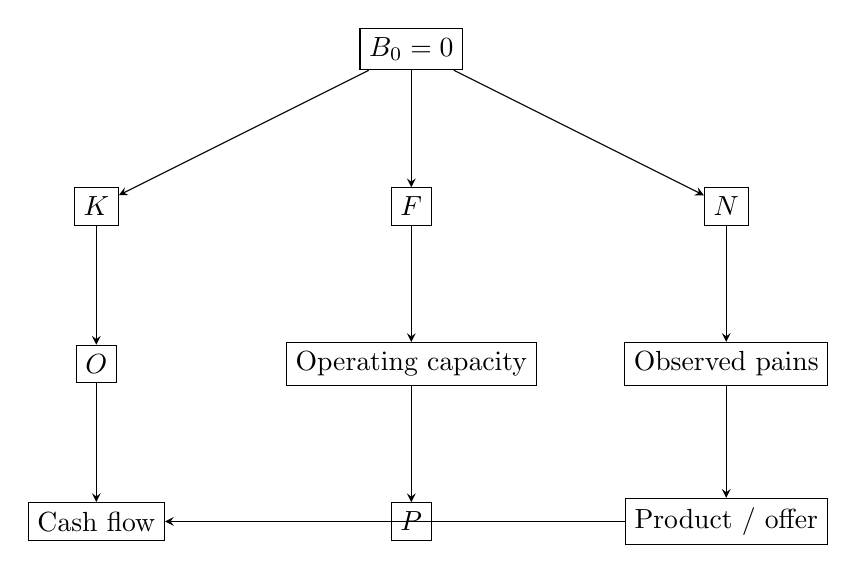
\begin{tikzpicture}[>=stealth]
\node[draw, rectangle] (b0) at (0,0) {$B_0=0$};

\node[draw, rectangle] (k) at (-4,-2) {$K$};
\node[draw, rectangle] (f) at (0,-2) {$F$};
\node[draw, rectangle] (n) at (4,-2) {$N$};

\node[draw, rectangle] (o) at (-4,-4) {$O$};
\node[draw, rectangle] (cap) at (0,-4) {Operating capacity};
\node[draw, rectangle] (prob) at (4,-4) {Observed pains};

\node[draw, rectangle] (cash) at (-4,-6) {Cash flow};
\node[draw, rectangle] (profit) at (0,-6) {$P$};
\node[draw, rectangle] (prod) at (4,-6) {Product / offer};

\draw[->] (b0) -- (k);
\draw[->] (b0) -- (f);
\draw[->] (b0) -- (n);

\draw[->] (k) -- (o);
\draw[->] (o) -- (cash);

\draw[->] (f) -- (cap);
\draw[->] (cap) -- (profit);

\draw[->] (n) -- (prob);
\draw[->] (prob) -- (prod);
\draw[->] (prod) -- (cash);
\end{tikzpicture}
\end{figure}

This figure is a reconstruction, not a photographed board. It simply keeps visible the three main recovery routes that the lecture puts on the table: skill, financing, and networked problem-finding.

\section{Rooms, Masterminds, and the Expansion of Belief}

After the zero-balance puzzle, the lecture makes a widening move. We have asked what remains in the individual; now we ask what changes when the room changes.

One answer is relational. Good people around you are not merely pleasant. They are accountability structures. They hold you to who you say you are, to the vision you claim to have, to the standards you intend to live by. They also create a healthy form of competition: not a race into vanity, but a sharpening.

The second answer is epistemic. When one sits at a table with people who are doing larger numbers, and hears those numbers described as ordinary reality, the possible becomes visible. The lecture repeats this in several ways: being in such a room shows that the outcome is real; it makes attainment imaginable; it expands the mind; it expands belief.

We may compress the mechanism into
\begin{equation}
N_{\mathrm{quality}} \uparrow
\;\Longrightarrow\;
B_{\mathrm{belief}} \uparrow
\;\Longrightarrow\;
X_{\mathrm{execution}} \uparrow,
\end{equation}
where \(N_{\mathrm{quality}}\) measures the quality of the room or network, \(B_{\mathrm{belief}}\) measures the effective range of outcomes that seem genuinely attainable, and \(X_{\mathrm{execution}}\) measures the range of action one can now undertake.

The lecture provides a concrete example. One speaker says his business used to stay around the lower edge of seven figures; after joining a mastermind, the next year brought a jump to ten million dollars. The essential claim is not magical. Advice became easier to access, but equally important, the ceiling of the imaginable moved. Self-limiting beliefs weakened because the room furnished evidence.

\section{Sales, Results, Personal Brand, and Recurring Revenue}

The lecture now narrows once more, this time from general commercial development to operating mechanics. The host asks first about the secret to sales, then about the secret to scale. The answers arrive in a compressed but coherent chain.

\paragraph{Rejection and reps.}
The first instruction is to be okay with rejection. Rejection is treated not as disproof of one's worth, but as information. From there the lecture moves immediately to repetition: get on as many calls as possible, because calls are reps, and reps improve performance. In notation,
\begin{equation}
n_{\mathrm{calls}} \uparrow
\;\Longrightarrow\;
n_{\mathrm{reps}} \uparrow
\;\Longrightarrow\;
p_{\mathrm{close}} \uparrow.
\end{equation}
This is heuristic rather than measured, but it is faithful to the lecture's logic. One interviewee explicitly links this to a sports background: repetition builds competence.

\paragraph{Results before image.}
The next answer is that sales should lead with results. In the agency example, credibility comes from demonstrated outcomes, not from verbal style alone. If the results are not there, the lecture endorses the uncomfortable but disciplined conclusion that the fit may simply be wrong. This is an important refinement: selling is not mere pressure; it is the commercialization of evidence.

\paragraph{Brand, content, and recurring revenue.}
Only then does the lecture ask the scaling question directly. The first part of the answer is top-of-funnel: build a personal brand, develop content, become comfortable on camera, and keep producing free value with consistency. These are trust and acquisition mechanisms.

The second part is the lecture's cleanest piece of unit economics. Let \(\mathrm{CAC}\) denote customer acquisition cost and \(\mathrm{LTV}\) denote customer lifetime value. Then the aggregate per-customer surplus is
\begin{equation}
\Pi_{\mathrm{cust}}=\mathrm{LTV}-\mathrm{CAC}.
\end{equation}
The interviewee's claim is that recurring revenue changes this quantity. If customers continue to pay over time, then the business no longer requires the first transaction to carry the whole burden of profitability.

A slightly more explicit reconstruction makes the point transparent. Suppose acquisition loses \(|\pi_0|\) initially, but recurring gross contribution \(m_t\) arrives over \(T\) periods. Then
\begin{align}
\Pi_{\mathrm{cust}}
&= -|\pi_0| + \sum_{t=1}^{T} m_t.
\end{align}
If, for a first approximation, the contribution is roughly constant, \(m_t \approx m\), then
\begin{align}
\Pi_{\mathrm{cust}}
&\approx -|\pi_0| + Tm.
\end{align}
Break-even occurs when
\begin{equation}
\Pi_{\mathrm{cust}} > 0
\;\Longleftrightarrow\;
Tm > |\pi_0|
\;\Longleftrightarrow\;
T > \frac{|\pi_0|}{m}.
\end{equation}

This is the mathematical core of the lecture's final claim. A business with recurring revenue can rationally tolerate an initially unprofitable acquisition, because the customer is not valued at the first transaction alone. That is why such a business can sometimes outspend a competitor on acquisition:
\begin{equation}
RR \uparrow
\;\Longrightarrow\;
\mathrm{LTV} \uparrow
\;\Longrightarrow\;
\mathrm{CAC}_{\max} \uparrow.
\end{equation}

The lecture's closing line about recurring revenue being a game changer is therefore not empty rhetoric. It is a statement about how the allowable acquisition budget changes once value is distributed over time.

\section{Summary}

The lecture begins with money as spectacle and ends with money as structure. We first hear annual income and revenue figures, then ask what those figures belong to, then ask what habits and skills make them reproducible, and finally ask what survives when cash disappears. The strongest answer is that wealth is not exhausted by stored money. It also lives in \(K\), in the ability to form \(O\), in the recognition of \(G\), in the quality of \(N\), and, at the scaling frontier, in the relation between \(\mathrm{CAC}\) and \(\mathrm{LTV}\). Read in that order, the lecture unfolds cleanly: shock, vehicle, principle, stress test, room, and then operating logic.